\section{Casos de uso}

\begin{figure}[H]
	\centering
	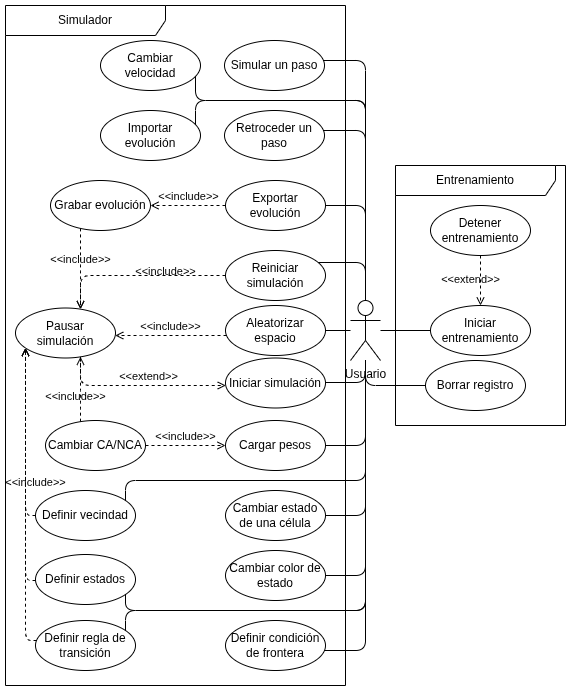
\includegraphics[width=0.95\linewidth]{img/uml_ucd.png}
	\caption{Diagrama de casos de uso}
	\label{fig:uml_ucd}
\end{figure}


\section{Diccionario}

\subsection{Interfaces gráficas}
\begin{itemize}
	\item \NewUI{control_ui}{Control}: Elemento que contiene los botones de control sobre la simulación del espacio celular.
	\item \NewUI{simulacion_ui}{Simulación}: Elemento que contiene la cuadrícula del espacio celular y muestra la evolución del autómata celular.
	\item \NewUI{configuracion_ui}{Configuración}: Elemento que permite realizar la configuración de la vecindad, condición de frontera, estados y función de transición.
	\item \NewUI{training_ui}{Entrenamiento}: Contiene la personalización del entrenamiento del autómata celular neuronal.
\end{itemize}

\subsection{Entradas}
\begin{itemize}	
	% Configuración
	\item Controles de simulación:
	\begin{itemize}
		\item \NewBTN{iniciar_simulacion}{Iniciar simulación}
		\item \NewBTN{pausar_simulacion}{Pausar simulación}
		\item \NewBTN{paso_adelante}{Simular un paso}
		\item \NewBTN{paso_atras}{Retroceder un paso}
		\item \NewBTN{reiniciar_simulacion}{Reiniciar simulación}
		\item \NewBTN{aleatorizar_simulacion}{Aleatorizar espacio}
		
		\item \NewBTN{importar}{Importar evolución}
		\item \NewBTN{grabar_evolucion}{Grabar evolución}
		\item \NewBTN{exportar}{Exportar evolución}
		
		\item \NewBTN{cargar_pesos}{Cargar pesos}
		\item \NewBTN{cambiar_ca_nca}{Cambiar CA/NCA}
	
		\item \NewSLD{velocidad}{Cambiar velocidad}
		\item \NewSLD{paso}{Eligir paso}
	
		\item \NewIN{grabar_pasos}{Numero de pasos}
	
		\item \NewMSG{formato_incorrecto}{Formato de archivo incorrecto}

		\item \NewMSG{tamaño_incorrecto}{Tamaño incorrecto}
		\item \NewMSG{evolucion_vacia}{Sin evolución}
	\end{itemize}
	
	\item Configuración del autómata celular:
	\begin{itemize}
		\item \NewBTN{def_vecindad}{Definir vecindad}
		\item \NewBTN{añadir_grupo}{Añadir grupo}
		\item \NewBTN{eliminar_grupo}{Eliminar grupo}
		
		\item \NewBTN{def_estados}{Definir estados}		
		\item \NewBTN{estado}{Estado $n$-esimo.}		

		\item \NewBTN{def_frontera}{Definir condición de frontera}
		
		\item \NewBTN{def_regla}{Definir regla}
		
		\item \NewIN{grupo_vecindad}{Grupo de vecindad}
		\item \NewIN{espacio_vecindad}{Espacio vecindad}
		
		\item \NewIN{estados}{Estados}		
		
		\item \NewIN{regla}{Regla}
		\item \NewIN{regla_codigo}{Regla (Código)}
	\end{itemize}
	
	\item Espacio de simulación:
	\begin{itemize}
		\item \NewIN{espacio}{Espacio}
	\end{itemize}
	
	\item Entrenamiento del automata celular neuronal:
	\begin{itemize}
		\item \NewBTN{cargar_evolucion}{Cargar evolución}
		\item \NewBTN{definir_guardado}{Definir ruta de guardado}
		
		\item \NewBTN{entrenar}{Iniciar entrenamiento}
		\item \NewBTN{detener}{Detener entrenamiento}
	
		\item \NewIN{entrenamiento_vecindad}{Vecindad}
		\item \NewIN{capas_ocultas}{Capas ocultas}
		\item \NewIN{neuronas}{Neuronas}
		\item \NewIN{relu}{Activación ReLU}
		\item \NewIN{sigmoid}{Activación sigmoide}
		\item \NewIN{tanh}{Activación Tanh}
		\item \NewIN{lineal}{Activación lineal}
		\item \NewIN{salida}{Capa de salida}
		\item \NewIN{funcion_salida}{Ultima función de activación}
		\item \NewIN{epocas}{Epocas}
		\item \NewIN{tamaño_lote}{Tamaño de lotes}
		\item \NewIN{tasa_aprendizaje}{Tasa de aprendizaje}
		\item \NewIN{perdida_objetivo}{Perdida objetivo}
		\item \NewIN{imprimir}{Imprimir cada N}
		
		\item \NewIN{borrar_consola}{Borrar consola}
		
		\item \NewMSG{entrenamiento_incompleto}{Entrenamiento incompleto}
		
		\item \NewOUT{ruta_in}{Ruta de evolución}
		\item \NewOUT{ruta_out}{Ruta de guardado}
		\item \NewOUT{entrenamiento_vecindad_mapa}{Mapa de vecindad}
		\item \NewOUT{consola}{Consola}
	\end{itemize}
\end{itemize}